% TODO: Extract to settings.tex

\chapter{An ADER-DG scheme for the Navier-Stokes Equations}\label{chap:methods}
This chapter describes the numerical and physical background that is needed to simulate reacting fluids with good accuracy.
We start with a description of the arbitrary high order derivatives (\ader{}) discontinuous Galerkin (\dg{}) method with a focus on equations that contain both advective and diffusive terms.
We then seque into a short description of the \muscl{} scheme which is a second order finite volume scheme.

e conclude this chapter by a description of finite volume limiting and adaptive mesh refinement (\amr{}).
The limiting combines both numerical methods to achieve a stable, high-order method and the \amr{} allows us to perform high quality simulations with a smaller computational cost.

\section{Reactive Compressible Navier Stokes Equations}\label{sec:navier-stokes}
\newcommand{\diffCoeff}{\varepsilon}
\newcommand{\hyperFluxDef}{
  \begin{pmatrix}
    \Qj \\
    \Qv  \otimes \Qj + \bm{I} \pressure  \\
    \Qv \cdot (\bm{I} \QE + \bm{I} \pressure) \\
    \Qj \QZZ
  \end{pmatrix}
}
\newcommand{\viscFluxDef}{
  \begin{pmatrix}
     -\diffCoeff \gradient{\Qrho}\\
     \stressT (\Q, \gradQ)  \\
     \Qv \cdot \stressT (\Q, \gradQ) - \kappa \gradient{T}\\
     -\diffCoeff \gradient{\QZ}
   \end{pmatrix}
}

Fluid motion can be described by the compressible Navier Stokes equations.
We follow the description in~\cite{dumbser2010arbitrary} for the Navier Stokes part.
The coupling with the advection-diffusion-reaction equation follows~\cite{hidalgo2011ader} which describes this equation set for the one-dimensional case.
In the following, we will denote the spatial coordinates as $\bm{x} = \left( x,z \right)$ and $\bm{x} = \left( x,y,z \right)$ for the two and three-dimensional case respectively.
The variable $t$ corresponds to the current physical time.
We solve the \pde{} in the conservative form% \pcref{eq:conservation-law-gradient}
\begin{equation}
 \label{eq:equation-set} 
 \begin{array}{l}
 \text{mass cons.} \\
 \text{momentum cons.} \\
 \text{energy cons.} \\
 \text{cont.\ gas} 
\end{array}
:
\quad
  \pdv{}{t}
  \underbrace{
  \begin{pmatrix}
    \Qrho\\
    \Qj\\
    \QE\\
    \QZ
    \end{pmatrix}}_{\Q}
  +
  \divergence{
  \underbrace{
  \left(
   \underbrace{\hyperFluxDef}_{\hyperFlux(\Q)}
+
\underbrace{\viscFluxDef}_{\viscFlux(\Q, \gradQ)}
  \right)}_{\flux(\Q, \gradQ)}}
 =
  \underbrace{
  \begin{pmatrix}
    \source[\Qrho\phantom{\Qrho}]\\
    \source[\Qj]\\
    \source[\QE]\\
    \source[\QZ]
    \end{pmatrix}}_{\source(\Q, \bm{x}, t)}
\end{equation}
which describes the time evolution of variables $\Q$ with respect to a flux $\flux(\Q, \gradQ)$ and a source $\source(\Q)$.
The vector of conserved quantities is given by
\begin{equation}
  \label{eq:conserved-variables}
 \Q = \left( \Qrho, \Qj, \QE, \QZ \right),
\end{equation}
where $\Qrho$ is the density, $\Qj$ is the two or three-dimensional momentum, $\QE$ the energy density and $\QZ$ is the mass fraction of the chemical reactant.
The chemical reactant in our case is unburnt gas.

The rows of the equation are the conservation of mass, the conservation of momentum, the conservation of energy and the continuity equation of the reactant.
We split the flux into a hyperbolic $\hyperFlux(\Q)$ and a viscous part $\viscFlux(\Q, \gradQ)$
\begin{equation}
  \label{eq:flux}
  \flux(\Q, \gradQ) = \hyperFlux(\Q) + \viscFlux(\Q, \gradQ).
\end{equation}
The hyperbolic flux is given by
\begin{equation}
  \label{eq:hyper-flux}
  \hyperFlux(\Q) = \hyperFluxDef,
\end{equation}
which are the Euler equations coupled with an advection equation.
In this equation $\bm{a} \otimes \bm{b} = \bm{a} \bm{b}^\intercal$ is the Kronecker or outer product of two vectors $\bm{a}$ and $\bm{b}$.
The pressure $\pressure$ is given by the caloric equation of state of an ideal reacting gas
\begin{equation}
  \label{eq:eos}
  \pressure = (\gamma - 1) \left(\QE - \frac{1}{2} \left(\Qv \cdot \Qj \right)  - q_0 \QZ - gz \right).
\end{equation}
The term $q_0 \QZ$ is the chemical energy with the heat release $q_0$, the term $gz$ is the geopotential height.
The pressure is related to the temperature $T$ by the thermic ideal gas law
\begin{equation}
  \label{eq:temperature}
 \frac{\pressure}{\Qrho} = RT,
\end{equation}
where $R$ is the specific gas constant of a fluid.

The viscous flux is
\begin{equation}
  \label{eq:visc-flux}
  \viscFlux(\Q, \gradQ) = \viscFluxDef.
\end{equation}
where $\stressT$ and $(\kappa \nabla T)$ denote the stress tensor and heat flux respectively.
The viscous effects of the fluid are modeled by the stress tensor
\begin{equation}
  \label{eq:stress-tensor}
  \stressT(Q, \nabla Q) =
  \mu
  \left(
  \left(\nicefrac{2}{3} \divergence{\Qv} \right) -
  \left( \gradient{\Qv} + \gradient{\Qv}^\intercal \right)
  \right).
\end{equation}

We further introduce the ratio of specific heats $\gamma$ and the heat fraction for constant volume $c_v$ and constant volume $c_r$.
These constants are all fluid dependent and relate to each other and the gas constant by
\begin{align}
  \label{eq:fluid-constants}
  \begin{split}
  c_v &= \frac{1}{\gamma - 1} R \\
  c_p &= \frac{\gamma}{\gamma - 1} R\\
  R &= c_p - c_v\\
  \gamma &= \frac{c_p}{c_v}.
  \end{split}
\end{align}
\todo{Cite sth for this!}
We can then compute the heat conduction coefficient
\begin{equation}
  \label{eq:heat-conduction-coeff}
  \kappa = \frac{\mu \gamma}{\Pr} \frac{1}{\gamma - 1} R = \frac{\mu \gamma}{\Pr} c_v,
\end{equation}
where the Prandtl number $\Pr$ depends on the fluid.
% Sutherland's viscosity law:
% \begin{equation}
%   \label{eq:sutherland}
%  \mu(T)  = \mu_0 {\left(\frac{T}{T_0}  \right)}^{\beta} \frac{T_0 + C}{T + C}
% \end{equation}
% with \(\beta = 1.5\), \(C = \text{const.}\), reference temperature $T_0$ and reference viscosity $\mu_=$.
% Equal to
% \begin{align}
%   \lambda &= \frac{\mu_0 (T_0 + C)}{T_0^\beta} \\
%   \mu(T) &= \lambda \frac{T^\beta}{T + C},
% \end{align}
% where $\lambda$ is constant for a given fluid.

The maximal absolute eigenvalues for convective and viscous part in direction of a normal vector $\normal$ are
\begin{align}
  \begin{split}
    \maxConvEigen &= \left( \partial \bm{F}/\partial \bm{Q}\right) \cdot \normal = \vert \Qv_{\normal} \vert + c,\\
    \maxViscEigen &= \left( \partial \bm{F}/\partial \left( \nabla \bm{Q} \cdot \normal \right)\right) \cdot \normal =
    \max \left( \frac{4}{3} \frac{\mu}{\Qrho},
                        \frac{\gamma \mu}{\Pr \Qrho},
                        \diffCoeff \right)
  \end{split}
\end{align}
with velocity in direction of the normal $\Qv_{\normal}$ and speed of sound $c = \sqrt{\gamma R T }$.

We also support two different kind of optional source terms.
The first source term is gravity, given by
\begin{equation}\label{eq:source-gravity}
  \source[\Qj] = - g \bm{k} \cdot \Qj,
\end{equation}
where $g = 9.81$ and $\bm{k}$ is a unit vector pointing in $z$-direction\todo{Discuss $g$ either in pressure or scenario.}.

\newcommand{\backgroundPressure}{\overline{\pressure}}
\newcommand{\backgroundRho}{\overline{\Qrho}}
Some of our scenarios can be described as a pertubation of a background state that is initially in hydrostatic balance
\begin{equation}
  \label{eq:hydrostatic-balance}
  \pdv{}{z} \backgroundPressure{\left (z \right )} = -g \backgroundRho(z),
\end{equation}
where $\backgroundPressure$ and $\backgroundRho$ is the background pressure and density.
We now focus on the following part of the momentum equation (neglecting viscous effects) of \cref{eq:equation-set}
\begin{equation}
  \label{eq:momentum-equation}
  \pdv{\Qj}{t}+ \divergence{
    \Qv \cdot \left( \bm{I} \QE + \bm{I} \pressure \right)
  }
  =
  -g \bm{k} \cdot \Qrho.
\end{equation}
The background state \cref{eq:hydrostatic-balance} can be comparitively large and can thus diminish other parts of the flux due to numerical instabilities~\cite{muller2010adaptive}.
To avoid this, we split the pressure as $\pressure = \backgroundPressure(z) + \pressure' (\bm{x}, t)$ and the density as $\Qrho = \backgroundRho(z) + \Qrho'(\bm{x}, t)$.
Inserting this splitting and the definition of divergence into \cref{eq:momentum-equation} allows us to apply \cref{eq:hydrostatic-balance}.
Furthermore, the background states have zero derivatives in all directions but in $z$.
We arrive at 
\begin{equation}
  \label{eq:momentum-equation-split}
  \pdv{\Qj}{t}+ \divergence \left(
    \Qv \cdot \left( \bm{I} \QE + \bm{I} \pressure' \right)
   \right)
  =
  -g \bm{k} \Qrho'.
\end{equation}.
We thus cancel parts of the flux with parts of the source term.
Note that the time derivative of the background density also vanishes.
This form of the equation is inspired by equation set 3 of~\cite{giraldo2008study}.
They additionally use a splitting of the energy and use the pertubations directly as conservative variables.
%We do not use this to simplify the implementation of gradients.

The chemical reactive source term is
\begin{equation}\label{eq:source-reaction}
  \source[\QZ] = - K(T) \QZ.
\end{equation}
We use the simple reaction model
\begin{equation}\label{eq:reaction-model}
\begin{cases}
  - \frac{1}{\reactionTimescale} & T > \reactionTemperature\\
  0 & \text{otherwise}
\end{cases}  
\end{equation}
where $\reactionTimescale$ is the timescale of the reaction and $\reactionTemperature$ is the activation temperature~\cite{hidalgo2011ader,helzel2000modified}.
\subsection{Boundary conditions}
To close the system we need to impose boundary conditions.\todo{Adapt this chapter to implementation!}

\sidetitle{Cauchy}
For some scenarios we use Cauchy boundary conditions, i.e.\ we prescribe both $\Q$ and $\gradQ$ at the boundary.
In most cases, we would like to impose periodic boundary conditions, due to the inner workings of \exahype{} this is not possible.
Instead we use the analytical solution of our problems at the boundary, imposing both value and gradients of the conservative variables.
Note that this leads to an error when our problem does not posses an exact analytical solution.
This is the case for test cases that are analytical solutions to the incompressible Navier Stokes equations but do not satisfy the compressible equation set.

As a physical boundary condition we limit ourselves to wall boundary condition

\sidetitle{No-Slip}
A standard wall boundary condition for viscous fluid is the no-slip condition, where we assume that the fluid has a velocity of zero near the wall.
\todo{Check if this is the correct physical description!}
We enfore this by setting
\begin{align}
  \label{eq:no-slip}
  \begin{split}
  \Qrho^o &= \Qrho^i, \\
  \Qj^o &= -\Qj^i, \\
  \QE^0 &= \QE^i,\\
  {(\nabla Q)}^o &= {(\nabla Q^o)},
  \end{split}
\end{align}
where a superscript of $o$ and $i$ denotes the values outside and inside of the boundary respectively.

\sidetitle{Free-Slip}
Similarly to the no-slip condition, we define the free-slip condition
\begin{equation}
  \label{eq:free-slip}
  \Qj^o_d = \begin{cases}
    -\Qj^i_d & d = \text{normal} \\
    \Qj^i_d & \text{otherwise}
    \end{cases}
\end{equation}
where only the velocity in normal direction is zero after the Riemann solver.
The other variables are extrapolated in the same manner as in \cref{eq:no-slip}.

We manually set the energy component of the numerical flux to zero for both no- and free-slip conditions.
\section{The ADER-DG Method}\label{sec:ader-dg}
\newcommand{\NVar}{N^{\text{var}}}
\newcommand{\dimensions}{d}
\newcommand{\mapping}{\mathcal{M}}
\newcommand{\volume}{V}
\newcommand{\cellCenter}{\operatorname{cell-center}}
We describe the arbitrary derivative discontinous Galerkin (\aderdg) method in this chapter.
Our description of the main method follows~\cite{dumbser2008unified,dumbser2010arbitrary,dumbser2018efficient}, our notation follows primarily~\cite{dumbser2018efficient}.
Let $\NVar$ be the number of variables, $\dimensions$ the number of spatial dimensions and $N > 0$ the order of the method.
We discuss the approximation of systems of partial differential equations (\pde) of the form
\begin{equation}
  \label{eq:conservation-law-gradient}
 \frac{\partial}{\partial_t}  \Q + \div \flux(\Q, \gradQ) = \source(\bm{x}, t, \Q),
\end{equation}
which in contrast to hyperbolic conservation laws of the form
\begin{equation}
  \label{eq:conservation-law}
 \frac{\partial}{\partial_t}  \Q + \div \flux(\Q) = \source(\bm{x}, t, \Q)
\end{equation}
contain the gradient $\gradQ \in \mathbb{R}^{\NVar \times \dimensions}$ of the so called vector of conservative variables $\Q \in \mathbb{R}^{\NVar}$~\cite{dumbser2010arbitrary}.
They are therefore not hyperbolic but rather parabolic or elliptic.

We discuss the solution of a conservation law \cref{eq:conservation-law-gradient} with two or three dimensional domain $\domain$ and boundary $\boundary$.
In our implementation of the discontinous Galerkin (\dg) framework, we approximate this solution in the space
\begin{equation}
  \label{eq:dg-space}
  \broken = \bigcup_k \cell[k]
\end{equation}
of disjoint quadrilateral cells $\cell$.
Note that we do not distinguish between the broken approximation space and the domain, the use should be clear given its surrounding context.
For each cell we denote its center by $\cellCenter{\cell}$ and its size by $\Delta x, \Delta y$ and $\Delta z$.

The \aderdg{}-scheme is a predictor-corrector method.
We first compute a local time evolution of each cell in a predictor step and then add the influence of the neighbors in the corrector step.
% \begin{algorithm}[H]
%   \begin{algorithmic}
%     \Let{$\stpredictor$}{Initial guess}
%     \Let{$F_h$}{$\flux(\Q, \gradQ)$}
%     \Let{$\stpredictor$}{Solve \cref{eq:space-time-predictor} using $F_h, \Q, \gradQ$}
%     \Let{$\left( \hat{F_h}, \hat{\Q}, \hat{\gradQ}, \hat{\stpredictor} \right)$}
%         {Extrapolate to boundary using \cref{eq:boundary-extrapolation}}
%     \Let{update}{Use \cref{eq:corrector} with boundary extrapolated values (fluxes of neighbors)}
%   \end{algorithmic}
%   \caption{The \textsc{ader-dg} algorithm for one cell.}
% \end{algorithm}

\sidetitle{Reference Cell}
For reasons of computational efficiency, we describe the scheme in terms of a reference cell.
We use the quad cell $\hat{\cell} = (0, 1)^\dimensions$ as space reference cell.
The mapping, which takes a point on the reference cell with coordinates $\hat{\bm{x}}$ and and returns a the coordinates $\bm{x}$ in a grid cell $\cell$ is
\begin{equation}\label{eq:space-mapping}
  \bm{x} = \mapping (\hat{\bm{x}}) =
  \cellCenter(\cell) +
\begin{pmatrix}
\Delta x && \\
&\Delta y & \\
&&\Delta z&
\end{pmatrix}
  \begin{pmatrix}
    \hat{x} - 0.5\\
    \hat{y} - 0.5\\
    \hat{z} - 0.5
  \end{pmatrix}.
\end{equation}
The inverse mapping $\mapping^{-1}$ can be used to define a function $f(\bm{x})$ acting on a point $\hat{\bm{x}}$ of a regular cell in terms of a function $\hat{f}(\bm{x})$ that acts on the corresponding point of the reference cell by the relation
\begin{equation}
  \label{eq:function-ref-cell}
  f(\bm{x}) = f\left( \mapping^{-1}(\bm{x}) \right) = \hat{f}(\hat{\bm{x}}).
\end{equation}

Similar to this, we define a mapping that maps a reference time point $\hat t$ to simulation time $t$
\newcommand{\timeMapping}{\mathcal{T}}
\begin{equation}
  \label{eq:time-mapping}
  t = \timeMapping(\hat{t}) = \curTime + (\Delta t) \hat{t},
\end{equation}
where the reference time interval is $[0,1]$ and the time interval of a cell is $[\curTime, \nextTime]$.
The time at the beginning of a timestep is thus denoted by $\curTime$, the time at the end of a step is denoted by $\nextTime = \curTime + \Delta t$ with timestep size $\Delta t$.

The Jacobian determinant of $\mapping$ is simply the volume $V$ of the cell
\begin{equation}
  \label{eq:determinant-mapping}
  \volume = \operatorname{det}(\operatorname{Jacobian}\mapping) = \Delta x \, \Delta y \,\Delta z,
\end{equation}
the Jacobian determinant of $\timeMapping$ is $\Delta t$.
This is useful for evaluating derivatives by the chain rule and, similarly, integrals by substitution.
For example, we can evaluate a volume integral over a cell by
\begin{equation}
  \label{eq:integration-by-substitution}
  \intdcell{
f(\bm{x})
  }
  =
\volume \intdrefcell{
    \hat{f}(\hat{\bm{x}})
  }
\end{equation}
\sidetitle{Basis Functions}
The next step is the definition of basis functions for our cells.
We use Langrange polynomials that are defined in the one-dimensional case for the reference interval $(0,1)$ by
\begin{align}
  \label{eq:lagrange-basis}
    \lagrangeRef(x) = \prod_{i >0, j>0, i \neq n}^N \frac{x - {\quadNode[j]}}{x_i - \quadNode[j]},
\end{align}
We can then approximate functions as a sum over the support points $\quadNode[j]$
\begin{equation}
  \label{eq:langrange-expansion-1d}
  f(x) = \sum_{i = 0}^N f(x_i) \lagrangeRef[i](x) = f(x_i) \lagrangeRef[i](x),
\end{equation}
where we used the Einstein summation convention which implies summation over repeated free indices.
This convention is used from here on.
The support points $\quadNode[i]$ are chosen such that they coincide with the nodes of the Gauss-Legendre quadrature of order $N+1$ which we can use to evaluate integrals
\begin{equation}
  \label{eq:quadrature-1d}
  \int_0^1 f(\hat{x}) \dd{\hat{x}} = \sum_{i=0}^{N} \quadWeight[i] f(\quadNode[i]),
\end{equation}
where $\quadWeight[i]$ is the quadrature weight corresponding to the node $\quadNode[i]$.

The basis functions are similarly defined in $\dimensions$-dimensions by considering nodes that are the tensor-products of $d$ one-dimensional Gauss-Legendre quadrature.
They are indexed by a multi-index $n = (n_1, \ldots, n_\dimensions)$
\begin{equation}
  \label{eq:basis-space}
  \sbasisRef[][n] (\bm{x}) = \prod_{i=0}^{\dimensions} \lagrangeRef[n_i] (x_i)
\end{equation}
that is linearised such that $n = (0, \ldots, \sbasisSize)$.
A $d$-dimensional function is then approximated by
\begin{equation}
  \label{eq:lagrange-expansion}
  f(\bm{x}) = \sum_{i = 0}^{\sbasisSize - 1} f(\bm{x}_i) \lagrangeRef[i](\bm{x}) = f(\bm{x}_i) \lagrangeRef[i](\bm{x}).
\end{equation}
Similarly to the one-dimensional case, we can evaluate integrals by
\begin{align}
  \label{eq:quadrature}
  \underbrace{\int_0^1 \cdots \int_0^1}_{\dimensions \text{ times}} f(\hat{\bm{x}}) \dd{\hat{\bm{x}}} &=
 \sum_{n=0}^{\sbasisSize-1} \quadWeight[n] f(\quadNodeNd[n]) \\
  \intertext{with}
  \quadWeight[n] &= \prod_{i}^{d} \quadWeight[n_i],
\end{align}
where the quadrature weights $\quadWeight[n]$ are the product of all relevant one-dimensional quadrature weights, using the aforementioned (linearized) multi-index $n$.
\todo{Should be correct. Is there a way to avoid this index hell, esp.\ multi-index?}

Two important properties of this family of polynomials are
  \begin{alignat}{10}
    \label{eq:basis-interpolating}
&& \text{Interpolating:} \qquad && \lagrangeRef[i] (\quadNode[j]) &= \delta_{ij},\\
&& \qquad && \sbasisRef[][n] (\quadNodeNd[m]) &= \delta_{nm}, \notag\\
\label{eq:basis-orthogonality}
&& \text{Orthogonality:} \qquad && \int_0^1 \lagrangeRef[i](x) \lagrangeRef[j](x) \dd{\hat{x}} &= \quadWeight[i] \delta_{ij},\\
&& \qquad &&
\underbrace{\int_0^1 \cdots \int_0^1}_{d \,\text{times}}
\sbasisRef[][n] \left( \hat{\bm{x}} \right)
\sbasisRef[][m] \left( \hat{\bm{x}} \right) \dd{\hat{\bm{x}}}
&= \quadWeight[n] \delta_{nm}, \notag
    \end{alignat}
    where we make use of the Kronecker delta
\begin{equation}
      \label{eq:kronecker-delta}
      \delta_{ij} =
      \begin{cases}
        1 & \text{if } i = j\\
        0 & \text{otherwise}
      \end{cases}.
\end{equation}
\todo{Fix this for multiple integrals!}

We define the basis functions over a space-cell with an index $n = 0, \ldots, \sbasisSize - 1$
\begin{align}\label{eq:space-basis}
  \begin{split}
  \sbasis[][n] (\bm{x}) &= \sbasisRef[][n] \left( \mapping(\bm{x}) \right)
  \end{split}
\end{align}
where $\sbasisRef$ denotes the basis function on the reference cell.

In addition to the space cells, we also introduce space-time cells $\cell \times [\curTime, \nextTime]$ with reference cell $(0,1)^\dimensions \times  [0,1]$.
A basis for these cells is given by
\begin{align}\label{eq:space-time-basis}
  \begin{split}
  \stbasisRef[][l,n](\hat{\bm{x}}, \hat{t}) &= \lagrange[l](t) \sbasis[][n] (x)\\
  \stbasis[][l,n] (\bm{x}, t) &= \stbasisRef \left( \mapping(\bm{x}), \timeMapping(t) \right)
  \end{split}
\end{align}
where the first index $l = 0, \ldots, N$ runs over times.
Outside of elements, we define the basis functions to be equal to 0.

We introduce an additional index $v = (0, \ldots, \NVar - 1)$ that corresponds to a variable.
The complete basis functions are then defined by
\begin{align}
  \stbasis[][v,n,l] (\bm{x},t)= \bm{I} \otimes \stbasis[][n,l] (\bm{x}, t)
\end{align}
with the identity matrix $\bm{I} \in \mathbb{R}^{\NVar}$\todo{Write out definition for space-time basis+both reference basis funcs. Explain kronecker delta, maybe when first used in pde chapter}.

\sidetitle{Expansion of quantities}
All quantities can be expanded in the space-time basis.
For example, the expansion of space-time predictor $\stpredictor[\cell]$ can be written as
\begin{equation}
  \label{eq:cell-approx-space-time}
  \stpredictor[\cell] (\bm{x}, t) = \stpredictorCoeff[\cell][v',l',n'] \stbasis[\cell][v',l',n'](\bm{x}, t).
\end{equation}
We denote the space-time flux as $\stflux$ and the space-time source as $\stsource$ with coefficient vectors $\stfluxCoeff$ and $\stsourceCoeff$.
Similarly, we define the space degrees of freedoms by an expansion in the space basis, for example for the space predictor
\begin{equation}
  \label{eq:cell-approx-space}
  \spredictor[\cell] (\bm{x}) = \spredictorCoeff[\cell][v',n'] \sbasis[\cell][v',n'] (\bm{x}),
\end{equation}
where the basis, unlike in \cref{eq:cell-approx-space-time}, does not depend on the time.
We need the space-expansion for the predictor $\spredictor$, the discrete solution $\ssol$, the source $\ssource$ and the flux $\sflux$,
with coefficients $\spredictorCoeff, \ssolCoeff, \ssourceCoeff$ and $\sfluxCoeff$ respectively.
The indices are in range of $v' = (0, \ldots, \NVar - 1)$, $n' = (0, \ldots, \sbasisSize - 1)$ and $l' = ( 0, \ldots, N)$.

Here, the computational advantage of the nodal approach is evident:
The coefficients correspond to the quantity evaluated at the basis node, due to the interpolation property~\pcref{eq:basis-interpolating}.

\sidetitle{Predictor}
We are now ready to derive the predictor.
We first multiply the conservation law by a test function of the same function space as the basis, integrate over a space-time-element $\cell$ and replace all terms with the discrete approximations.
In particular, we replace the vector of conservative variables $\Q$ with the space-time predictor $\stpredictor[\cell]$.
\begin{equation}\label{eq:weak-pde-space-time}
\intdt{\intdcell{
    \sttestfunction[\cell][v,l,n](\bm{x}, t)
    \pdv{\stpredictor}{t}
}}
+
\intdt{\intdcell{
    \sttestfunction[\cell][v,l,n](\bm{x}, t)
    \left(
      \divergence{\stflux(\stpredictor, \gradient{\stpredictor})}
    \right)
}}
=
\intdt{\intdcell{
  \sttestfunction[\cell][v,l,n] \stsource(\bm{x}, t, \stpredictor)
}},
\end{equation}
where the indices $v = (0, \ldots, \NVar-1)$, $n = (0, \ldots, \sbasisSize - 1)$ and $l = (0, \ldots, N)$ run over the variables, space and time.

Henceforth, we drop the cell index for all quantities and the spatial argument for the basis and test functions.
We integrate the first term of \cref{eq:weak-pde-space-time} by parts in time and the flux divergence in space.
Here we do not use the Riemann solver for the flux boundary term but rather use the known discrete solution at time $t$.
This corresponds to upwinding in time~\cite{dumbser2008unified}.
Note that this neglects the interaction with neighbouring cells.
The cell-local scheme is then
\begin{align}\label{eq:space-time-predictor}
\begin{split}
\intdcell{
  \sttestfunction[][v,l,n] (\nextTime) \stpredictor(\nextTime)
}
&-
\intdt{\intdcell{
    \pdv{}{t} \sttestfunction[][v,l,n] (t) \stpredictor(t)
}}
= \\
\intdcell{
  \sttestfunction[][v,l,n] (\curTime) \ssol (\curTime)
}
&+
\intdt{\intdcell{
    \sttestfunction[][v,l,n] (t) \divergence{\stflux(\stpredictor, \gradient{\stpredictor})}
}}
+
\intdt{\intdcell{
    \sttestfunction[][v,l,n] (t) \stsource(\stpredictor)
}}.
\end{split}
\end{align}

Using the expansions in space and time~\pcref{eq:cell-approx-space,eq:cell-approx-space-time} results in a local systems of equations that can be solved by a fixed-point iteration scheme.
For the space-time predictor, we introduce an iteration counter $i$.
To close the iterative scheme, we set the initial value for the space-time predictor as
\begin{equation}
  \label{eq:initial-guess}
\forall l: \quad \stpredictorCoeff[i][v,l,n] = \ssolCoeff[v,n]
\end{equation}
which corresponds to a stationary initial guess~\cite{dumbser2008unified}.
For an overview of possible initial guesses, see~\cite{dumbser2018efficient}.

To show the computational efficiency of our scheme, we follow the approach of~\cite{dumbser2008unified} and collect our integrals into matrices\todo{Maybe mention that they are actually unrolled tensors?\\Source here is Dominics \aderdg{}-document.}.
We arrive at the cell-local scheme
\begin{align}
  \label{eq:predictor-iterative}
  \pleft \stpredictorCoeff[i+1] &= \prightsol (\ssol) - \prightpred(\stpredictorCoeff[i]) \\
 \stpredictorCoeff[i+1] &= \pleft^{-1} \left( \prightsol (\ssol) - \prightpred(\stpredictorCoeff[i]) \right).
\end{align}
where we introduced the matrices
\begin{equation}
  \label{eq:matrices}
  \pleft \in \mathbb{R}^{\NVar \stbasisSize \times \NVar \stbasisSize}, \quad
  \prightsol \in \mathbb{R}^{\NVar \stbasisSize}, \quad
  \prightpred \in \mathbb{R}^{\NVar \stbasisSize}
\end{equation}
with entries
\begin{align}
  \label{eq:predictor-matrices}
\begin{split}
  \pleft_{(v l n), (v l' n')} &=
\intdcell{
  \sttestfunction[][v,l,n](\nextTime) \  \stbasis[][v,l',n'](\nextTime)
}
\\&-
\intdt{\intdcell{
  \left( \pdv{}{t} \sttestfunction[][v,l,n] (t) \right) \stbasis[][v,l',n'] (t)
}}
\end{split}
\\
\begin{split}
\prightsol_{v,l,n} (\ssol) &=
\intdcell{
  \sttestfunction[][v,l,n] (t) \sbasis[][v,n'] \ssolCoeff[][v,n']
}
\\&+
\intdt{\intdcell{
  \sttestfunction[][v,l,n] (t) \stbasis[][v,l',n'](t) \stsourceCoeff[][v,l',n'](\stpredictor[i])
}}                             
\end{split}
  \\
\prightpred_{v,l,n} (\stpredictor) &=
\stfluxCoeff[][v,l',n'] (\stpredictor)
\intdt{\intdcell{
  \left( \gradient{\sttestfunction[][v,l,n]} \right) \stbasis[][v,l',n'](t)
}}
\end{align}
Note here that $\prightpred$ is constant during a interation step.
In practice, we precompute all integrals that contain only basis functions and their derivatives for the reference cell.
The computation of the integrals for general space-tiem cells can then be done by \cref{eq:integration-by-substitution}.
For details and proof of convergence for case of linear \pde{}s, see~\cite{dumbser2008unified}.

\sidetitle{Preparing for corrector}
It is useful to precompute time-averaged versions of our quantities.
For example, this can be done for the space-time predictor by
\begin{align}\label{eq:time-average}
  \begin{split}
  \spredictor (\bm{x}) &= \frac{1}{\Delta t} \intdt{
\stpredictor(\bm{x}, t),
  } \\
\spredictor[][v,n] (\bm{x}) &= \stpredictorCoeff[][v,l,n] \quadWeight[l].
  \end{split}
\end{align}
We then extrapolate the space predictor and its gradient, and the fluxes to the boundary.
In our case we have a $\dimensions - 1$ dimensional basis for all $2 \dimensions$ faces.
We accomplish this by evaluating the function at the degrees of freedom at the boundary.
Due to the interpolating property of the nodal basis~\pcref{eq:basis-interpolating}, this reduces to a change of basis which can be precomputed on the reference element.
We use the extrapolated values later for the Riemann solver and for the reconstruction of boundary values.

\sidetitle{Corrector}
The final step of the \aderdg{}-scheme is the corrector.
We multiply the system \cref{eq:conservation-law-gradient} by a space test function $\stestfunction$ and integrate over the space-time control volume.
This results, yet again, at the weak formulation of the \pde{}
\begin{equation}
  \label{eq:weak-pde}
\intdt{\intdcell{
\stestfunction[][v,n] \pdv{\Q}{t}
}}
+
\intdt{\intdcell{
    \stestfunction[][v,n] \left( \div{F(\Q, \gradQ } \right)
}}
=
\intdt{\intdcell{
    \stestfunction[][v,n] S(\Q, \bm{x}, t)
}}.
\end{equation}
We now insert our discrete approximations and apply the basis expansions \cref{eq:cell-approx-space,eq:cell-approx-space-time} to the space-time predictor.
The first part can be integrated by parts in time with the convenient result that only the boundary terms remain because the basis is constant in time.
We then integrate the flux divergence by parts in space and insert the Riemann solver to connect with the neighbouring elements.
Finally, we need to solve\todo{Fix notation, is tensor not matrix}
\newcommand{\massMatrixDef}{\intdcell{
  \stestfunction[][v,n] \sbasis[][v,n']
}}
\begin{align}
\begin{split}
\label{eq:corrector}
\left(
\massMatrixDef
\right)
(\ssolCoeff[t^{n+1}][v,n'] - \ssolCoeff[t^n][v,n'])
&+
\left(\intdt{\intdcellb{
      \stestfunction[][v,n] \Riemann(\stpredictor[-], \gradient{\stpredictor[-]}; \stpredictor[+], \gradient{\stpredictor[+]}) \cdot \normal
}}\right)
-\\
\left(\intdt{\intdcell{
    \gradient{\stestfunction[][v,n]} \cdot  \stflux(\spredictor, \gradient{\spredictor})
}}\right)
&=
\left(\intdt{\intdcell{
      \stestfunction[][v,n] \stsource(\spredictor)
}}\right)
\end{split}
\end{align}
for the coefficients $\ssolCoeff[\nextTime][v,n]$ of the new solution.
Here the superscripts $\pm$ denotes values that are extrapolated to the boundaries.
Again, the computational effort can be vastly reduced by collecting the integrals into matrices and precomputing as much as possible.
The first term is the mass tensor with entries
\newcommand{\massMatrix}[1][]{\bm{M}_{#1}}
\begin{equation}
  \label{eq:mass-matrix}
  \massMatrix[v n n'] = \massMatrixDef = \volume \underbrace{\quadWeight[n] \delta_{n n'}}_{\text{diagonal}}
\end{equation}
which is, due to the orthogonal basis \pcref{eq:basis-orthogonality}, diagonal for each variable $v$ and thus trivial to invert.
We can then insert the definition of our basis function into our equation and arrive at
\begin{align}
  \massMatrix \left( \ssolCoeff[t+1] - \ssolCoeff[t] \right) &=
  \Delta t \left( \bm{a} - \bm{b} + \bm{s} \right) 
  \intertext{with}
a_{v,n} &= \sfluxCoeff[][n'] \intdcell{
  \sbasis[][v,n'] \gradient{\sbasis[][v,n]}(t)
}
\\
\label{eq:corrector-surface}
b_{v,n} &= \intdcellb{
    \stestfunction[][v,n] \Riemann \left( \spredictor[-], \gradient{\spredictor[-]}; \spredictor[+], \gradient{\spredictor[+]} \right) \cdot \normal
} \\
s_{v,n} &=
\ssourceCoeff[][v,n'] \intdcell{
  \sbasis[][v,n] \sbasis[][v,n']
}
,
\end{align}
where we evaluated the time-integrals by \cref{eq:integration-by-substitution}.
All quantities are now time-averaged~\pcref{eq:time-average} and are represented in the space basis~\pcref{eq:cell-approx-space}.
Note that we evaluate the Riemann problem for the time-averaged space-predictor.
This is justified by the linearity of our numerical flux~\cite{dumbser2008unified,dumbser2010arbitrary}.
The surface integral \pcref{eq:corrector-surface} can be evaluated by summing over the contributions of the faces of each cell, which are computed by integrating the extrapolated space predictor with Gaussian quadrature.
Finally, we can solve \cref{eq:corrector} for the new unknows $\ssolCoeff[k+1]$
\begin{align}\label{eq:update-predictor}
\begin{split}
  %\bm{u}^{n+1}
  \ssolCoeff[k+1][v]
  &= \ssolCoeff[k][v] + \Delta t (\operatorname{update}) \\
  \operatorname{update} &= \massMatrix[v]^{-1} \left( \bm{a}_v - \bm{b}_v + \bm{s}_v \right)
\end{split}
\end{align}
which is clearly of the form of a one-step scheme.

\sidetitle{Riemann solver \textit{\&} timestep}
As a Riemann solver we use a simple Rusanov-flux that is adapted for diffusive problems
\begin{equation}
  \label{eq:rusanov-flux}
  \Riemann(q_h^-, \nabla q_h^-; g_h^+, \nabla q_h^+) \cdot \bm{n} =
  \frac{1}{2} \left(
    F(q_h^+, \nabla q_h^+) +
    F(q_h^-, \nabla q_h^-)
  \right) -
  \frac{1}{2} s_\text{max} (q_h^+ - q_h^-),
\end{equation}
with a penalty term
\begin{equation}
  \label{eq:parabolic-penalty}
  s_\text{max}  = \max \left(
\maxConvEigen[q_h^-], \, \maxConvEigen[q_h^+]
\right) +
2 \eta \max \left(
\maxViscEigen[q_h^-], \, \maxViscEigen[q_h^+]
\right)
\end{equation}
and
\begin{equation}
  \eta = \frac{2N+1}{h \sqrt{\frac{1}{2} \pi}}.
\end{equation}
In this equation $h$ is the side-length of an element.
The penalty term depends on the maximal absolute eigenvalues of both the convective and viscous part of the equations
\begin{align}
  \begin{split}
    \maxConvEigen &= \left( \partial \bm{F}/\partial \bm{Q}\right) \cdot \normal,\\
    \maxViscEigen &= \left( \partial \bm{F}/\partial \left( \nabla \bm{Q} \cdot \normal \right)\right) \cdot \normal,
  \end{split}
\end{align}
in direction of the normal vector $\normal$ to the cell face. 

This Riemann solver was first published in~\cite{gassner2008discontinuous} and used for an \textsc{ader-dg} scheme in~\cite{dumbser2010arbitrary}.
\todo{Paper only describe 1d}
The timestep per dimension $d$ is restriced to a so-called \textsc{cfl}-type penalty
\begin{equation}\label{eq:cfl-aderdg}
 %\Delta t \leq  \text{CFL} \, \frac{\alpha(N) \, h}{\maxConvEigen + 2 \maxViscEigen \frac{1}{\alpha(N) h}}
 \Delta t \leq  \text{CFL} \, \alpha(N) \, h \sum_{i=0}^{\dimensions-1} \frac{1}{\maxConvEigen + 2 \maxViscEigen \frac{1}{\alpha(N) h}},
\end{equation}
where the eigenvalues are evaluated for the flux Jacobian in direction $i$~\cite{dumbser2010arbitrary,gassner2008discontinuous}..
The constant $\alpha(N) \leq {\left( 2N+1  \right)}^{-1}$ is obtained from von Neumann analysis on a simple model problem and depends on the approximation order~\cite{dumbser2008unified}.
We use this constant for both hyperbolic and diffusive penalty terms to ensure stability.
For a more detailed and rigoruous stability analysis of the Riemann solver, see~\cite{gassner2008discontinuous}\todo{Is this the correct paper, or is this in the other part of the series?}.
We use a value of $0.7$ for the constant $\text{CFL}$.

\section{MUSCL-Hancock Finite Volume Scheme}\label{sec:muscl}
\todo{Mention dubious treatment of viscous boundary terms. Or later in exahype chapter.}
\newcommand{\cellAvg}[1][i,j]{U_{#1}}
\newcommand{\sign}{\operatorname{sign}}
\newcommand{\minmod}{\operatorname{minmod}}
\newcommand{\slope}[2][i,j]{s^{#2}_{#1}}
\newcommand{\gradCellAvg}[1][i,j]{\gradient{\cellAvg[#1]}}
\newcommand{\fluxX}{\flux_x}
\newcommand{\fluxY}{\flux_y}
We discussed a modern, high-order \dg{} method in the previous chapter.
While this scheme is efficient, it can become unstable, especially in case of discontinuities.
A simple alternative is a finite volume scheme.
We use the \muscl{} method\todo{Cite original paper (van Leer)}.
Our discussion and notation follows the one in~\cite{toro2009riemann}.
Similar to~\cite{toro2009riemann} we only describe the two-dimensional case, an extension to three dimensions is straigthforward.
\todo{Source term!}

In contrast to the previous \dg{} scheme, we now only store averages instead of a full polynomial solution for each cell.
We achieve higher order then by reconstructing a linear function from a cell and its neighbours.
Let $\cellAvg$ denote the averages per cell at spatial coordinates $i,j$.

\sidetitle{Boundary Extrapolated Values}
We first compute the slope of the linear function connecting the cells.
We use the minmod slope-limiter
\begin{equation}
  \label{eq:minmod}
  \operatorname{minmod}(a, b) =
  \begin{cases}
    0.0 & \sign(a) \neq \sign(b) \\
      a & \vert a \vert < \vert b \vert \\
      b & \text{otherwise}
  \end{cases}
\end{equation}
to avoid unphyiscally steep gradients and to stabilize the system~\cite{leVeque2002finite}.
This function can be used to compute the slopes
\begin{align}\label{eq:slopes}
  \begin{split}
   \slope{x} &=  \Delta x \minmod \left( \cellAvg[i+1,j] - \cellAvg[i,j], \, \cellAvg[i,j] - \cellAvg[i-1, j] \right),\\ 
   \slope{y} &=  \Delta y \minmod \left( \cellAvg[i,j+1] - \cellAvg[i,j], \, \cellAvg[i,j] - \cellAvg[i, j-1] \right),
   \end{split}
\end{align}
where $\Delta x$ and $\Delta y$ are the inverse cell sizes in $x$ and $y$ direction respectively.

We use the slope to reconstruct the value at the boundary.
In the following, $\cellAvg^{\pm x}$ is the average of the left ($+$) or right ($-$) cell boundary.
Similar, $\cellAvg^{\pm y}$ is the value at the top/bottom cell boundary.
These so called boundary extrapolated values are given by
\newcommand{\extrapolatedCellAvg}[3][i,j]{\cellAvg[#1]^{#3 #2} = \cellAvg #3 \frac{1}{2} \slope{#2}}
\begin{equation}
\begin{alignedat}{2}
& \extrapolatedCellAvg{x}{-} , \qquad && \extrapolatedCellAvg{x}{+}, \\
& \extrapolatedCellAvg{y}{-} , \qquad && \extrapolatedCellAvg{y}{+}.
\end{alignedat}
\end{equation}
We also use the slopes defined in \cref{eq:slopes} to estimate the gradient of $\cellAvg$ in each cell by the block matrix
\begin{equation}
  \label{eq:muscl-gradient}
  \gradCellAvg = \left( \slope{x} \bigg\rvert \slope{y} \right),
\end{equation}
which is of course an abuse of notation insofar as it is not the gradient of the constant cell value but rather of the linear reconstruction \pcref{eq:slopes}.
\sidetitle{Time Evolution}
To achieve second order in time, we evolve the boundary extrapolated values
\newcommand{\evolvedCellAvg}[2][i,j]{\hat{U}_{#1}^{#2}}
\begin{equation}\label{eq:muscl-time-evolution}
  \begin{split}
  \forall (k \in \{-x, +x, -y, +y \} ): \quad  \hat{U}_{ij}^k = \cellAvg^k &+
  \frac{\Delta t}{2 \Delta x} \left[ \fluxX(\cellAvg^{-x}, \gradCellAvg) - \fluxX(\cellAvg^{+x}, \gradCellAvg) \right] \\&+
  \frac{\Delta t}{2 \Delta y} \left[ \fluxY(\cellAvg^{-y}, \gradCellAvg) - \fluxY(\cellAvg^{+y}, \gradCellAvg) \right],
  \end{split}
\end{equation}
where $\fluxX$ and $\fluxY$ denote the $x$ and $y$ part of the flux respectively.
Note that we do not need to consider neighboring cells for this step.

Finally, the update can be described by\todo{Double check update}
\begin{align}
  \begin{split}
    \cellAvg (t^{n+1}) &= \cellAvg (t^n)
    \\ &+
  \frac{\Delta t}{\Delta x}
    \Riemann \left(
      \evolvedCellAvg[i-1,j]{+x}, \gradCellAvg[i-1,j]; \ %
      \evolvedCellAvg[i,j\phantom{-1}]{-x}, \gradCellAvg[i,j\phantom{-1}]
    \right)
    \\ &-
  \frac{\Delta t}{\Delta x}
    \Riemann \left(
      \evolvedCellAvg[i,j\phantom{+1}]{+x}, \gradCellAvg[i,j\phantom{+1}]; \ %
      \evolvedCellAvg[i+1,j]{-x}, \gradCellAvg[i+1,j]
    \right)
    \\ &+
  \frac{\Delta t}{\Delta y}
    \Riemann \left(
      \evolvedCellAvg[i,j-1]{+y}, \gradCellAvg[i,j-1]; \ %
      \evolvedCellAvg[i,j\phantom{-1}]{-y}, \gradCellAvg[i,j\phantom{-1}]
    \right)
    \\ &-
  \frac{\Delta t}{\Delta y}
    \Riemann \left(
      \evolvedCellAvg[i,j\phantom{+1}]{+y}, \gradCellAvg[i,j\phantom{+1}]; \ %
      \evolvedCellAvg[i,j+1]{-y}, \gradCellAvg[i,j+1]
    \right).
  \end{split}
\end{align}
This results in a scheme that has an order of convergence of two for both space and time.

We again use the Rusanov-type Riemann solver~\cref{eq:rusanov-flux}.
The timestep is subject to a penalty of the form
\begin{equation}\label{eq:cfl-muscl}
 \Delta t \leq  \text{CFL} \, \frac{h}{\maxConvEigen + 2 \maxViscEigen \frac{1}{h}},
\end{equation}
with a constant value of CFL that is typically close to $0.7$.

\section{Adaptive Mesh Refinement \textit{\&} Finite Volume Limiting}\label{sec:grid}
This section is concerned with two different but related concepts:
finite volume limiting and adaptive mesh refinement (\amr{}).
Both have in common that they change the structure of the grid.
Instead of a regular grid where each cell has the same size, we now have different cell sizes.

\subsection{Limiting}\label{sec:limiting}
Higher order \textsc{dg} methods cannot cope with discontinuous solutions.
Even worse, in the case of non-linear fluxes, discontinuities can appear even from smooth initial data.
In addition, oscillations stemming from the high-order polynomical approximation can lead to wrong or unphyiscal data.
This is called Gibbs phenomenon.
A classical way of dealing with this problem is the usage of so called limiters.
The idea is to smooth out steep gradients and thus lessen the effect of discontinuities~\cite{hesthaven2008nodal}.

A relatively recent way of dealing with this problem is the finite volume subcell limiter.
Our discussion follows the one in~\cite{dumbser2016simple}.
This limiting is an a posteriori limiting, which means that we first evaluate a timestep with an unlimited \aderdg{}-method and then check, whether our solution is \enquote{correct}.
In our case, we check whether the solution is a finite floating point number.
We also check whether it is physically admissible with the criterion\todo{Do I actually check for pos.\ of Z?}
\begin{equation}
  \label{eq:limiting-physical}
  \operatorname{is-admissible}(\Q) =
  \begin{cases}
    \text{true} & \Qrho > 0 \land \pressure > 0 \land \QZZ > 0 \\
    \text{false} & \text{otherwise}.
  \end{cases}
\end{equation}
The positivity of the pressure implies positivity of energy.

\todo{Reread dmp description, fix formulas.}
To combat the Gibbs phenomenon, we can make use of the discrete maximum principle (\textsc{dmp}).
This criterion marks cells as troubled that have a numerical solution that is significantly higher or lower than the solutions of its neighbours.
\begin{align}\label{eq:limiting-dmp}
\min (u(y, t^{\curTime})) - \delta &\leq u^*(y, t^{\nextTime}) \leq \max (u(y, t^{\curTime})) + \delta
%
%
\intertext{with tolerance}
\delta &= \max \left(
  \varepsilon_0, \varepsilon \left(
         \max(u(y,t^{\curTime})) -
         \min(u(y,t^{\curTime}))
  \right)
  \right)
\end{align}
The parameters $\varepsilon$ and $\varepsilon_0$ can be set freely.
The former is controls by which factor the local jump can differ from its neighbourhood, the latter is needed for zero jumps~\cite{dumbser2016simple}.
Note that this criterion is suspectible for false positives, this is especially a problem in the presence of a source term.
\todo{Mention problems with source term?}

If a solution violates our criterion, we recompute the last timestep for the offending cells with a limited finite volume method.
In our case we use the \muscl{}-method (\cref{sec:muscl}).
The recomputation starts by subdividing the infringing cell into $N_s = 2N + 1$ subcells.
This number of subcells has the advantage that we do not lose spatial resolution and that we can use the same timestep size for both cell types.
The reason for this is that the \textsc{cfl}-conditions for both schemes \pcref{eq:cfl-aderdg,eq:cfl-muscl} coincide for our choice of $N_s$.
\begin{figure}[htb]
  \centering
  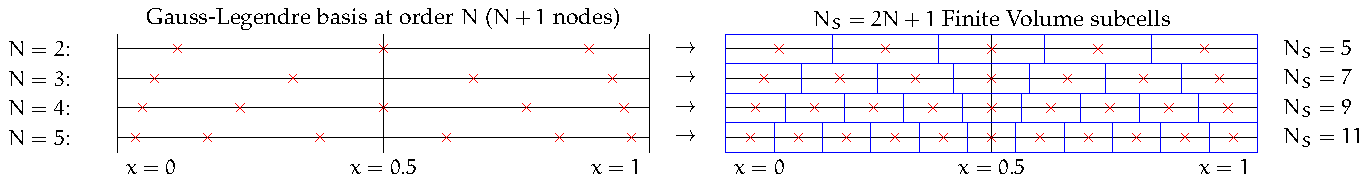
\includegraphics[scale=0.7]{thesis_aderdg_subcell_grid}
  \caption{\label{fig:limiting-subcells}Conversion from \dg{} degrees of freedoms to finite volume degree of freedoms. Image taken from~\cite{dumbser2018conformal}. }
\end{figure}
\todo{Cite source for subcells~\pcref{fig:limiting-subcells}. See guidebook. NOTE THAT IT IS MODIFIED. Also: Fix size, currently font is too small}

\Cref{fig:limiting-subcells} depicts the mapping from \dg{}-cells to finite volume subcells.
For the sake of brevity, we omit technical details and refer the interested reader to~\cite{dumbser2016simple}.

\subsection{Adaptive Mesh Refinement}\label{sec:amr}
The goal of \amr{} is to increase the computational efficiency by using a coarse spatial resolution in areas with low information content and a higher resolution in areas of interest.
A simple example for this would be using finer mesh cells for the simulation of a wave, while using a low resolution for areas where the wave does not pass through.
Of course, the difficult part is defining areas of interest.
We use a global, gradient based refinement strategy.
We first describe the computation of our indicator variable and then describe a simple way how one can detect outliers.

Let $\bm{f}(\bm{x}): \mathbb{R}^{N_\text{vars}} \to \mathbb{R}$ be a function that maps the discrete solution of a cell to an arbitrary indicator variable.
Furthermore, we assume that $\bm{f}$ is expanded in the space-basis \pcref{eq:cell-approx-space}.
Then the total variation (\textsc{tv}) of this function is defined by\todo{Cite sth for this?}
\newcommand{\tv}{\operatorname{TV}}
\begin{equation}
  \label{eq:tv}
  \tv \left[ f(\bm{x}) \right] =
  \Vert
\intdcell{ \vert \gradient{f \left( \bm{x} \right)} \vert }
\Vert_1
,
\end{equation}
for each cell.
The operator $\Vert \cdot \Vert_1$ denotes the discrete $l_1$ norm in this equation.
This integral can be evaluated efficiently on the reference cell \pcref{eq:space-mapping,eq:cell-approx-space} with Gaussian quadrature \pcref{eq:quadrature}.

\todo{Definition for FV schemes (maybe just mapping to DG-Cells)}
\newcommand{\gobs}{\operatorname{G}}
\newcommand{\mean}{\mu}
\newcommand{\std}{\sigma}
\newcommand{\variance}{\std^2}
\newcommand{\gobsCount}{n}
\newcommand{\sampleVariance}{\overline{\variance}}
A simple way of determining outliers is by how many standard deviations a value differs from the mean value.
We thus want to compute the mean and variance over all grid cells.
For computational efficiency and to simplify the implementation, we do this by performing only pairwise merge operations.
The simplest way to compute is by the textbook definitions of mean $\mean$ and population variance $\variance$ of a random variable $X$
\newcommand{\expectation}{\mathbb{E}}
\begin{align}
  \begin{split}
    \mean [X] &= \expectation \left[ X \right],\\
    \variance [X] &= \expectation \left[ X^2 \right] - \expectation \left[ X \right]^2,
  \end{split}
\end{align}
where $\expectation \left[ X \right]$ denotes the expectation of a random variable $X$.
The naive algorithm is numerically unstable when the variance is orders of magnitudes smaller than the mean, as this can lead to catastrophic cancellations.
We thus compute the mean and variance with the parallel algorithm of~\cite{chan1982updating}.
To do this, we need to store three variables per computation unit:
the mean $\mean$, the current sample variance $\sampleVariance$ and the number of processed elements $n$.
We collect these items in the vector $\gobs = (\mean, \sampleVariance, \gobsCount)$.
We can then merge a pair of observed variables with \cref{alg:merge-variance}.
This algorithm computes an estimate of the population variance using Bessel's correction, i.e.\ it returns the sample variance times $\nicefrac{n}{n-1}$.
In our case, the compute the variance over all grid cells.
This is why we compute the population standard deviation by
\begin{equation}
  \label{eq:sample-std}
 \sigma = \sqrt{ \frac{n-1}{n} \sampleVariance}.
\end{equation}
\begin{algorithm}[ht]
  \begin{algorithmic}
% TODO: Special cases 
\Function{reduce-variance}{$\gobs_0, \gobs_1$}
\If{$\gobsCount_0 = 0$}
  \State\Return{$\mean_1, \variance_1, \gobsCount_1$}
\EndIf\
\If{$\gobsCount_1 = 0$}
  \State\Return{$\mean_0, \variance_0, \gobsCount_0$}
\EndIf\
  \Let{$\Delta$}{$\mean_1 - \mean_0$}  
  \Let{$\gobsCount_\Sigma$}{$\gobsCount_0 + \gobsCount_1$}
  \Let{$m_a$}{$\variance_0 (\gobsCount_0 - 1)$}
  \Let{$m_b$}{$\variance_1 (\gobsCount_1 - 1)$}
  \Let{$m_\Sigma$}{$\nicefrac{m_a + m_b + (\Delta^2 \gobsCount_0 \gobsCount_1)}{\gobsCount_\Sigma}$}
  \Let{$\mean_\Sigma$}{$\mean_0  \gobsCount_0 + \mean_1 \gobsCount_1$}
  \State\Return{$
    \nicefrac{\mean_\Sigma}{\gobsCount_\Sigma},
    \nicefrac{m_\text{total}}{\gobsCount_\Sigma - 1},
    \gobsCount_\Sigma
    $}
\EndFunction\
  \end{algorithmic}
  \caption{\label{alg:merge-variance}
    Merging two sets of reduced mean and variance~\cite{chan1982updating}}
\end{algorithm}
Chebychev's inequality
\begin{equation}
  \label{eq:chebychev}
  \mathbb{P}(\vert X - \mu \vert \geq c \sigma) \leq \frac{1}{c^2},
\end{equation}
where $\mathbb{P}$ is the probability of an event,
holds for arbitrary distributions with mean $\mu$ and standard deviation $\sigma$~\cite{wasserman2004all}.
This motivates the following refinement criterion
\begin{equation}
  \label{eq:refinement-criterion}
  \operatorname{evaluate-refinement}(\Q, \mu, \sigma) =
  \begin{cases}
    \text{refine} & \text{if } \tv(\Q) \geq \mu + T_\text{refine} \sigma \\
    \text{delete} & \text{if } \tv(\Q) < \mu + T_\text{delete} \sigma \\
    \text{keep} & \text{otherwise}
    \end{cases}
\end{equation}
which refines a cell when its total variations differs by a multiple of the standard deviation.
In this equation, the constants $T_\text{refine}$ and $T_\text{delete}$ can be used to tailor the trade-off between the quality of approximation and computational cost.
They can be chosen freely, as long as $T_\text{refine} < T_\text{delete}$.
Chebychev's inequality~\pcref{eq:chebychev} then guarantees that only a subset of cells is marked for refinement.
Note that this inequality provides only a loose bound.
If one would be willing to assume a distribution of the indicator variable, tighter bounds can be derived~\cite{wasserman2004all}.

%%% Local Variables:
%%% mode: latex
%%% TeX-master: "../main"
%%% End:
